\documentclass[12pt]{article}

%%%%%%%%%%%%%%%% Commands for including graphics %%%%%%%%%%%%%%%%%%%
\usepackage{graphicx}
\DeclareGraphicsExtensions{.ps,.eps,.pcx}
%%%%%%%%%%%%%%%%%%%%%%%%%  End of these commands %%%%%%%%%%%%%%%%%
\usepackage{amsmath}
\usepackage{amssymb}

%\usepackage{mathtools}
%\usepackage{dsfont}
\usepackage{latexsym}
\usepackage{eucal}
\usepackage{color}
\usepackage{multirow}
\usepackage{enumitem}
\setlist{nolistsep}

\usepackage{algorithm}
\usepackage{setspace} % spacing in the algorithm
\usepackage{listings} % code Darstellung

\lstset{ 			  % code style
	backgroundcolor=\color{white},
	keepspaces=true,
	numbers=left,						% where to put the line-numbers
	numberstyle=\tiny\color{black},
	stepnumber=1,						% the step between two line-numbers
	captionpos=b,						% sets the caption-position to bottom
	tabsize=2,  						% sets default tabsize to 2 spaces
	showstringspaces=false,				% underline spaces within strings or not
	columns=flexible,
	%breaklines=true					% enter is breakline
	basicstyle={\small\ttfamily},		% the size of the fonts that are used 
	keywordstyle=\color{blue},
	commentstyle=\color{mygreen},
	stringstyle=\color{red},
	escapeinside={\%*}{*)},
	morekeywords={*,...}
}
\definecolor{mygreen}{rgb}{0,0.6,0}

\textwidth16cm

\textheight23cm

\oddsidemargin0.25cm

\evensidemargin0.25cm

\parindent0.4cm
\parskip2ex plus0.5ex minus0.5ex
\renewcommand{\baselinestretch}{1.37}
\unitlength1.0cm \headheight0cm \topskip0cm \headsep-1cm
%

%\newcommand{\cov}{\mbox{cov\,}}
%\newcommand{\var}{\mbox{var\,}}
%\newcommand{\bbo}{\mbox{1}\hspace{-3pt}\mbox{I}}
%\renewcommand{\Re}{\mbox{I}\hspace{-2pt}\mbox{R}}

\newtheorem{definition}{Definition}
\newtheorem{theorem}{Theorem}
\newtheorem{corollary}{Corollary}
\newtheorem{proposition}{Proposition}
\newtheorem{lemma}{Lemma}
\newtheorem{remark}{Remark}
\newtheorem{example}{Example}

\renewcommand{\thetheorem}{\arabic{theorem}.}
\renewcommand{\thedefinition}{\arabic{definition}.}
\renewcommand{\thecorollary}{\arabic{corollary}.}
\renewcommand{\theremark}{\arabic{remark}.}
\renewcommand{\theproposition}{\arabic{proposition}.}
\renewcommand{\thelemma}{\arabic{lemma}.}

\newcommand\inner[2]{\langle #1, #2 \rangle}

\newcommand{\bbo}{\mbox{1}\hspace{-3pt}\mbox{I}}
\newcommand{\Na}{\mbox{I}\hspace{-2pt}\mbox{N}}

\newcommand{\real}{\mbox{I}\hspace{-2pt}\mbox{R}}
\newcommand{\indi}{\mbox{1}\hspace{-3pt}\mbox{I}}
\newcommand{\B}{\mbox{I}\hspace{-2pt}\mbox{B}}
\newcommand{\intplus}{\mbox{I}\hspace{-2pt}\mbox{N}}
\newcommand{\integer}{\mbox{Z}\hspace{-4pt}\mbox{Z}}
\newcommand{\F}{\mbox{I}\hspace{-2pt}\mbox{F}}
\newcommand{\var}{\mbox{var\,}}
\newcommand{\Var}{\mbox{Var\,}}
\newcommand{\Cov}{\mbox{Cov\,}}
\newcommand{\cov}{\mbox{cov\,}}

\newcommand{\bbbr}{\mbox{I}\hspace{-2pt}\mbox{R}}
\newcommand{\bbbn}{\mbox{I}\hspace{-2pt}\mbox{N}}
\newcommand{\bbbone}{\mbox{1}\hspace{-3pt}\mbox{I}}
\newcommand{\bbbz}{\mbox{Z}\hspace{-4pt}\mbox{Z}}

% Define some commands to keep the formatting separated from the content 
\newcommand{\keyword}[1]{\textbf{#1}}
\newcommand{\tabhead}[1]{\textbf{#1}}
\newcommand{\code}[1]{\texttt{#1}}
\newcommand{\file}[1]{\texttt{\bfseries#1}}
\newcommand{\option}[1]{\texttt{\itshape#1}}

%---------------------------------------------------------------------------------------
%	BIBLIOGRAPHY SETTINGS
%---------------------------------------------------------------------------------------

\usepackage[backend=bibtex,style=authoryear,natbib=true]{biblatex} % Use the bibtex backend with the authoryear citation style (which resembles APA)

\addbibresource{NameMeBIB.bib} % The filename of the bibliography

\usepackage[autostyle=true]{csquotes} % Required to generate language-dependent quotes in the bibliography

%---------------------------------------------------------------------------------------

\begin{document}

%Dependence structures and central limit theorems of
%Theoretical results
\title{Partial analysis of the spatial ESEMFIAR model}
\author{Sebastian Letmathe and Jim Luca Brand\\ Faculty of Business Administration and Economics,
%Department of Economics, 
Paderborn University}
\maketitle
%\doublespacing

%\centerline{\large $^3$Swiss Federal Research Institute WSL}

\begin{abstract}

\noindent 
 A  spatial SEMIFAR model is defined by introducing a smoothing component into the spatial FARIMA model. The application of this model to non-negative financial data via log-transformation is hence called spatial ESEMIFAR. This model is analyzed by partially applying the ESEMIFAR model to univariate financial time series, namely on all observations at a given trading day and on observations of all days at a given trading time. After elimination of a deterministic trend conditional fluctuations in both dimensions are further investigated. The estimation of the nonparametric component can be simply carried out through SEMIFAR-algorithms. The appropriateness of our approach is then investigated and illustrated by the application to financial high-frequency data. Trend estimation and model selection is implemented with the statistical software R. 
 
\vspace{.3cm}

\noindent{\it Keywords:}  S-FARIMA, S-SEMIFAR, long memory, random fields, high-frequency data, local polynomial


\vspace{.3cm}

\noindent{\it JEL Codes:} C14, C51
\end{abstract}
\newpage

\section{Introduction}
Literature research and model research required.\\
\\ 
In many areas of research data are observed spatially, depending on two separate dimensions in a lattice. 
In recent years one can observe more frequently some sort of apparent memory in the decay of spatial correlations to depend and change over its direction within the spatial process. 
For instance, long-memory in the sense of slowly decaying autocorrelations in (high frequency) financial data across trading time and trading day produces a random field on a lattice in both dimensions simultaneously. 
\textcite{beran2015modelling}
state that daily average trade duration data has often shown long memory
with a clear non zero mode. Therefore a log-normal conditional distribution is suggested.
The simplest approach to model long range dependence in a positive valued
time series is to take the exponential of a linear long memory process such as
FARIMA leading to stochastic volatility models. Due to the long range dependence
there is an unobservable latent process which makes the estimation and interpretation
of the fitted parameters very challenging.\\
\\
The SEMIFAR and ESEMIFAR models introduced by \textcite{beran2002semifar} and \textcite{beran2015modelling} are designed for simultaneous modeling of stochastic trends, deterministic trends and stationary short- and long-memory components in a time series such that the trend generating mechanisms can be distinguished.
%A process \(Y_{t}\) is said to follow a SEMIFAR model introduced by 
%if there exists an integer \(m \in \{0,1\}\) and a fraction \(\delta\in (-0.5,0.5) \) such that 
%\begin{equation}
%\label{eq:3.1}
%\phi(B)(1-B)^{\delta} \{(1-B)^m Y_t - g(x_t)\}= \epsilon_t,
%\end{equation} 
%where \(\phi(x) = 1 - \sum_{j=1}^{p} \phi x^{j} \) is a polynomial with all roots outside the unit circle, iid. \( \epsilon_t \) with \(E(\epsilon_t) = 0\), var\((\epsilon_t) = \sigma_{\epsilon}^{2} \) and \( t \in \mathbb{Z} \).
%The one dimensional \(x_t\) is as in \eqref{eq:S-SEMIFAR} which incorporates \eqref{eq:3.1} as a special case.
%A SEMIFAR process has long memory if \eqref{eq:2.1e} and \eqref{eq:2.1f} are satisfied which requires the autocovariances \( \gamma(k) \) to behave proportional to \(k^{2\delta - 1}\) producing an infinite sum of autocovarinces for \(k \rightarrow \infty \). 
%Since the trend is non parametric and not assumed to follow a particular form   \eqref{eq:3.1} includes stochastic trends for \(m > 0\) where the differenced process can show short- or long memory components, and deterministic trends for \(m = 0\) with stationary short- or long memory components.
%Hence \(g(x_t)\) is allowed to be a constant (e.g. the mean) or a smooth function with a stochastic and/or a deterministic trend. 
%Consequently under \(m = 0\) a  continuous trend plus stationary noise admits a spurious trend, 
%whereas for  \(m > 0\) and \(g \neq 0 \) the trend is generated simultaneously by a deterministic and a stochastic trend. 
%Then the differenced process without the trend is a stationary fractional ARIMA process. 
Following \textcite{beran2015efarima} we assume \(X_{t}\) is some daily (average duration) series. 
Using  a clearly defined structural condition to avoid an unobservable latent process leads us to a multiplicative error model (MEM) in line with \textcite{engle2002new} of the form 
\begin{equation}
\label{eq:5.8} X_{t} = \nu\lambda_{t}\eta_{t},
\end{equation}
including a scale parameter \(\nu > 0\).
The \(\lambda_{t} > 0\) gives the conditional mean of the rescaled error \(X_{t}/\nu\) determined by the \(\sigma\)-algebra of past observations and the \(\log(\eta_{t}) = \epsilon_{t}\) are iid. random variables, such that \(\eta_{t} \sim N(0,\sigma_{\epsilon}^{2})\) are log normal distributed (other distributions are also possible). Taking logs of the MEM yields according to \textcite{beran2014empirical}
\begin{equation}
\label{eq:5.9}
Y_{t} = \mu(x_t) + Z_{t},
\end{equation} 
where 
$
Z_{t} = \log(\lambda_{t}\eta_{t}) = \zeta_{t} + \epsilon_{t}
$
gives the structural assumption and formulates the exponential transformation made in \eqref{eq:5.8}.
The notation \(\log(X_{t}) = Y_{t} \), \(\log (\nu) = \mu\), \(\log(\lambda_{}) = \zeta_{t}\) and \(\log(\eta_{t}) = \epsilon_{t}\) relates the equations \eqref{eq:5.8}, \eqref{eq:5.9} and \eqref{eq:5.9c} respectively. 
Recall \eqref{eq:3.1} and notice that the constant mean \(\mu\) is replaced by a smooth trend \(g\) depending on \(x_t\).
The stochastic \(Z_{t}\) is by \textcite{beran2015modelling} assumed to follow a stationary zero mean fractional ARIMA(p,\( \delta \),q) process.
%we use a multiplicative error model (MEM) $ X_t = \nu \lambda_{t} \eta_{t} $
%as the exponential of \eqref{eq:S-SEMIFAR} and the notation for
%the scalar \(\nu = \exp(\mu)\) 
The scalar in the original process \eqref{eq:5.8} can be expressed as 
$\nu(x_{t}) = \exp(\mu(x_{t}))$
including a positive and nonparametric regression function \(\mu(x_{t})\).
Thus the series \(X_{t} = \exp(Y_{t})\) is given by
\begin{equation}
\label{eq:5.14}
X_{t} = \nu(x_{t})\lambda_{t}\eta_{t} = g(x_{t})\eta_{t},
\end{equation}
where \(X_{t}^{*}  = \lambda_{t}\eta_{t}\) is the stationary process for modeling long-range dependence with \(d > 0\) and is \(\sim \log N(0,\sigma^{2})\).
The total mean of the original \(X_{t}\) is given by the trend function 
$ g(x_{t}) = \nu(x_{t}) \lambda_{t} $,
which equals the product of the conditional mean \(\lambda_{t} > 0\) and the local mean function \(\nu(x_{t}) > 0\).   
A process described by \eqref{eq:5.14} is called an exponential SEMIFAR or ESEMIFAR process.
With suitable regularity conditions it is a locally stationary process following \textcite{dahlhaus1997fitting}. This specification allows different conditional distributions and accounts 	simultaneously for a slowly changing scale function along with short range and long range dependence. The model fit is omitted since the SEMIFAR implementation can be used. 

\section{Local polynomial regression with long memory}
Let \(Y_{t}\) be an equidistant and nonparametric additive regression model of the form
\begin{equation}
\label{eq:Start}
Y_{t} = g(x_{t}) + Z_{t},
\end{equation} 
with standardized time \(x_t = t/n\), a nonparametric smooth trend function \(g:[0,1]\) and some stationary process \(Z_t\) which is assumed to be fractionally differenced such that \((1-B)^{\delta}Z_t =U_t\) holds, where \(U_t = Z_t\) for short memory with \(\delta = 0\).
Therefore \(Z_t\) may be called a  fractional ARIMA or FARIMA(p,\(\delta\),q) process capturing persistent dependency and is given by 
\begin{equation}
\label{eq:FARIMA}
	(1-B)^{\delta}\phi(B) Z_{t} = \psi(B) \epsilon_{t}, 
\end{equation}
where the fractional memory parameter \( \delta \in (-0.5,0.5) \),
%integer differencing parameter in \((1-B)^{m}\) is \(m=0\), \(d = m + \delta = )
 \(B\) as backshift operator, \( \phi(B) = 1 - \sum_{k=1}^{p} \phi_{k} B^k \) and \( \psi(B) = 1 + \sum_{k=1}^{q} \psi_{k} B^k \) are the characteristic autoregressive and moving average polynomials for short memory and \( \epsilon_{t} \, (t \in \mathbb{Z}) \)  are iid. random variables with \(E(\epsilon_{t} = 0)\) and \(var(\epsilon_{t} = \sigma_{\epsilon}^{2})\).
The fractional differencing parameter \( \delta \) was introduced by \textcite{granger1980introduction} and \textcite{hosking1981fractional} and is defined by 
\begin{equation}
\label{eq:fractional difference 1}
(1-B)^{\delta} = \sum_{k=0}^{\infty} b_k(\delta) B^k, 
\end{equation} 
with
\begin{equation}
\label{eq:fractional difference 2}
b_k(\delta) = (-1)^{k}{\delta\choose k}  = (-1)^{k} \frac{\Gamma(\delta+1)}{\Gamma(k+1)\Gamma(\delta-k+1)}. 
\end{equation} 
Considering the autocovariances \(\gamma(k) = \text{cov}(U_t,U_{t+k})\), \(Y_t\) incorporates long memory if the spectral density of \(Z_t\) in \eqref{eq:Start} given by
\begin{equation}
\label{eq:long memory1}
f(\lambda) = \frac{1}{2 \pi} \sum_{k=-\infty}^{\infty} e^{i k \lambda} \gamma(k) 
\end{equation}
and exhibits a pole at the origin of the frequency spectrum such that
\begin{equation}
\label{eq:long memory2}
f(\lambda) \sim c_f |\lambda|^{-2\delta}, \quad (\text{as}\, \lambda \rightarrow 0)
\end{equation}
where \(c_f > 0\) is a nonzero positive constant and "\(\sim\)" indicates that the ratio of both sides converges to one. 
Then, for \(k \rightarrow \infty\) the autocovariances \( \gamma(k) \) are proportional to \(k^{2\delta - 1}\) and yield an infinite sum of autocovariances. 
In consequence we can distinguish between three temporal dependency structures.
%
The process \(Z_t\) in \eqref{eq:Start} has long memory for \(\delta > 0\) with \( \sum_{k=-\infty}^{\infty} \gamma_{U}(k) = \infty  \), short memory for \(\delta = 0\) with \( \sum_{k=-\infty}^{\infty} \gamma_{U}(k) < \infty  \)
and is anitpersistent for \(\delta < 0\) with \( \sum_{k=-\infty}^{\infty} \gamma_{U}(k) = 0  \) frequently reversing itself. 
%If \(f(\lambda)\) in \eqref{eq:2.1f} converges to the right hand expression with \(\delta = 0\), then \(Z_t\) in \eqref{eq:S-SEMIFAR} has short memory and a positive finite sum of autocovariances. 
%For \(\delta \in  (-0.5,0)\) the stationary process is antipersistent, frequently reversing itself. 
%If \eqref{eq:long memory1} holds with \(\delta \in (0,0.5)\), \(Z_t\) is said to have long range dependence. 
%The representation in \eqref{eq:S-SEMIFAR} is included in the SEMIFAR model (see \cite{beran2000data}).
%
A time series \(Y_t\) in \eqref{eq:Start} including a smooth component and a stationary persistent dependence structure 
can be described by a SEMIFAR(p,\(\delta\),\(0\)) process (\textcite{beran1998unified,beran2002semifar}), since \(Y_t\) (with \(q = 0\)) can be modeled such that
\begin{equation}
\label{eq:SemifarEquation}
	\phi(B)(1-B)^{\delta} \{(1-B)^m Y_t - g(x_t)\}= \epsilon_t,
\end{equation}
using an additive approach with nonparametric regression and long memory as a semiparametric extension of \eqref{eq:FARIMA}. 
Here \(m \in \left\lbrace 0,1 \right\rbrace \) gives the smallest possible integer for the estimation of differenced data.
%
A semiparametric process as in \eqref{eq:SemifarEquation} has long memory if \eqref{eq:long memory1} and \eqref{eq:long memory2} are satisfied which requires the autocovariances \( \gamma(k) \) to behave proportional to \(k^{2\delta - 1}\) producing an infinite sum of autocovarinces for \(k \rightarrow \infty \). 
Since the trend \( g(x_t) \) is non parametric and not assumed to follow a particular form, \eqref{eq:SemifarEquation} includes stochastic trends for \(m > 0\) where the differenced process can show short- or long memory components, and deterministic trends for \(m = 0\) with stationary short- or long memory components.
Hence \(g(x_t)\) is allowed to be a constant (e.g. the mean) or a smooth function with a stochastic and/or a deterministic trend. 
Consequently under \(m = 0\) a  continuous trend plus stationary noise admits a spurious trend, 
whereas for  \(m > 0\) and \(g \neq 0 \) the trend is generated simultaneously by a deterministic and a stochastic trend. 
Then the differenced process without the trend is a stationary fractional ARIMA process \eqref{eq:FARIMA}. 
Further reading as to the spectral density representation for the memory of a process can be found in \textcite{mandelbrot1983fractal,cox1984review,kunsch1987statistical,hampel1987data,beran1995maximum}. In particular, for long memory in random fields view \textcite{angulo2000estimation,anh1999possible}.\\
\\
%The general fractional differencing parameter \(\delta\) without an index is the power in the fractional difference of \textcite{granger1980introduction} and \textcite{hosking1981fractional} defined by 
%\begin{equation}
%\label{eq:2.1c}
%(1-B)^{\delta} = \sum_{k=0}^{\infty} b_k(\delta) B^k, 
%\end{equation} 
%with
%\begin{equation}
%\label{eq:2.1d}
%b_k(\delta) = (-1)^{k} \binom{\delta}{k}  = (-1)^{k} \frac{\Gamma(\delta+1)}{\Gamma(k+1)\Gamma(\delta-k+1)}. 
%\end{equation} 
%
%
For the estimation of a smooth \(g^{(\nu)}\) in \eqref{eq:Start} a local polynomial approach is investigated by \textcite{ruppert1994multivariate,wand1994kernel,fan1995data,beran2002local}.
A polynomial approximation of the unknown function \(g(x)\) is used for \(x\) in neighborhood of a point \(x_{t}\)
and is \((p+1)\) times differentiable. 
The local approximation of \(g(x)\) is following \textcite{beran2016long} and \textcite{beran2002local} given by the \(p\) order polynomial
\begin{equation}
\label{eq:2.1}
g(x_{t}) \approx g(x) + g^{(1)}(x)(x_{t} - x) + \ldots + g^{(p)}(x)\frac{(x_{t} - x)^{p}}{p!} + R_{p},
\end{equation}
with a remainder term \(R_{p}\). 
Applying a polynomial regression locally for the observations \(y_{1},\ldots,y_{n}\) and using \eqref{eq:2.1}, 
the \(\nu\)th derivative of the estimator of \(g^{(\nu)}(x)\) are given by
\(\hat{g}^{(\nu)}(x)= \nu! \hat{\beta}_{\nu}\) 
where the fixed coefficients \(\beta_{\nu} = \beta_{\nu}(x) = g^{(\nu)}(x) / \nu!\) 
with \(\nu = 0,1,2,\ldots,p\) 
such that \eqref{eq:2.1} becomes
\(g(x_{t}) = \sum_{\nu=0}^{p}(x_{t} - x)^{\nu} \beta_{\nu} \).
Assume the kernel \(K\) to be a symmetric density with compact support \([-1,1] \) such that (see \textcite{gasser1984estimating})
\begin{equation}
\label{eq:Kernelfunction}
K(x) = \sum_{l=0}^{r}\alpha_l x^{2l}, \quad (|x| \leq 1)   %\, \mathds{1}
\end{equation}
with \(K(x) = 0\) for any point \(|x| > 1\), \(r \in \left\lbrace0,1,2,\ldots \right\rbrace \) and the integral of \(K\) between \((-1,1)\) yields one. 
Then the estimator \(\hat{g}^{(\nu)}(x)\) with \((\nu \leq p)\) is obtained when the locally weighted sum of squared residuals is minimized such that
\begin{equation}
\label{eq:2.2}
Q(x) = \sum_{t=1}^{n} \left\lbrace y_{t} - \sum_{j=0}^{p} \beta_{j}(x_{t} - x)^{j} \right\rbrace^{2} K \left( \frac{x_{t} - x}{h} \right) \Rightarrow min ,
\end{equation}
with \(h\) as bandwidth and \(\hat{\beta} = (\hat{\beta}_{0},\hat{\beta}_{1},\ldots,\hat{\beta}_{p})^{T}\) and
the weight term \(K((x_{t} - x)/h)\) limits the farthest neighbor for the polynomial fit for \(x\).
%With  we have  \(\nu ! \beta_{\nu} = \hat{g}^{(\nu)}(x)\). 
The matrix representation of \eqref{eq:2.2} is 
\begin{equation}
\label{eq:2.3}
Q(x) = (\mathbf{y} - \mathbf{X}\beta)^{T} \mathbf{K}(x) (\mathbf{y} - \mathbf{X}\beta)  ,
\end{equation} 
with
$$
\mathbf{X} = \begin{bmatrix}
1   & x_1 - x &   \cdots  & (x_1 - x )^{p}  \\
\vdots & \vdots  & \ddots    & \vdots          \\
1   & x_n - x & \cdots    & (x_n - x )^{p}  \\
\end{bmatrix},
$$
and 
$$
\mathbf{K} = \begin{bmatrix}
K \left( \frac{x_{1}-x}{h}\right) & 0 								   & \cdots  & 0      \\
0 								  & K \left( \frac{x_{2}-x}{h}\right)  & \ddots  & \vdots \\
\vdots 							  & \ddots        					   & \ddots  & 0      \\
0   							  & \cdots 							   & 0  	 & K \left( \frac{x_{n}-x}{h}\right) \\
\end{bmatrix},
$$
leading to a solution of \eqref{eq:2.2} and \eqref{eq:2.3} and can according to \textcite{feng2004non} be written as
\begin{equation}
\label{eq:Trend}
\begin{split}
\hat{g}^{(\nu)}(x) = \nu!\hat{\beta}_{\nu} & = \nu! e_{\nu+1}^{T} (\mathbf{X}^{T} \mathbf{KX})^{-1} \mathbf{X}^{T} \mathbf{K} \mathbf{y} \\
& = \left\lbrace \mathbf{w}^{\nu}(x) \right\rbrace^{T} \mathbf{y},
\end{split}
\end{equation}
the \(p\)-th order local polynomial estimator \(\hat{g}^{(\nu)}\) with \(\mathbf{y} = (y_{1},\ldots,y_{n})^{T}\), the weighting system \(\left\lbrace \mathbf{w}^{\nu}(x) \right\rbrace^{T} = (w_{1}^{\nu},\ldots,w_{n}^{\nu})^{T} = \nu! e_{\nu+1}^{T} 
(\mathbf{X}^{T} \mathbf{KX})^{-1} \mathbf{X}^{T} \mathbf{K}\) and
using the unit vector \(e_{\nu} = (e_{1,\nu},\ldots,e_{(p+1),\nu})^{T}\) with
\(\nu = 1,\ldots,p+1\) where \(e_{\nu,\nu} = 1\), \(e_{i,\nu} = 0\) for \(i \neq \nu\).
The weighting system for any \(t\) is nonzero only if \(|x_{t} - x| \leq h\) and therefore all interior points within \([h,1-h]\) share the same \(w^{\nu}\) and are independent of the errors dependence structure. 
Furthermore the weights have under any design the properties
\begin{equation}
\label{eq:2.5}
\sum_{t=1}^{n} w^{\nu} (x_{t} - x)^{\nu} = \nu! \,\,\,\,\, \text{and} \,\,\,\,\,  \sum_{t=1}^{n} w^{\nu} (x_{t} - x)^{l} = 0,
\end{equation}
for \(l=0,\ldots,p\) where \(j\neq\nu\). Since \eqref{eq:2.5} yields \( 0 \)  except for \(l = \nu\), \(\hat{g}^{(\nu)}\) is unbiased if the polynomial is of maximal order \(p\). This relation is also true for not equidistant 
In consequence a local polynomial estimator is boundary corrected for odd \(p - \nu\) as the order of the bias for interior and boundary points is the same whereas kernel estimators only approximate the properties and encounter boundary point problems.
The calculation of the bias of \(\hat{g}^{(\nu)}(x)\) for \(p - \nu\) odd and even is omitted and can be seen in \textcite{beran2016long}.

\section{Extension of the SEMIFAR model} 
A spatial extension of the SEMIFAR model in \eqref{eq:Start} to a higher dimensional space is achieved 
by running \(Y_{t}\) over a second index \(j\) such that a random field on a lattice originates along the trading time \(j\) and the trading day \(t\).   
Let \(Y_{t,j}\) be an equidistant, spatial and nonparametric regression model of the form
\begin{equation}
\label{eq:S-SEMIFAR}
Y_{t,j} = g(x_{t},\tau_{j}) + Z_{t,j},
\end{equation} 
with a non negative random field, rescaled \(x_t = t/n_1\), \(\tau_j = j/n_2\) and a trend \(g(\cdot,\cdot) : [0,1] \rightarrow {\rm I\!R} \) which is a smooth lattice process.
The multivariate \(Z_{t,j}\) in \eqref{eq:S-SEMIFAR} is a stationary lattice process and assumed to follow a zero mean S-FARIMA model 
which was introduced by \textcite{beran2009least} in order to account for the two-dimensional anisotropic memory of a process and is expressed by 
%\eqref{eq:S-FARIMA}
%\begin{equation}
%\label{eq:2.1b}
%(1-B)^{\delta_1} (1-B)^{\delta_2}  X_{t,j} = U_{t,j},
%\end{equation}
%with \(\delta_1, \delta_2 \in (-0.5,0.5)\), \(E(Z_{t,j}) = 0\), \(Var(Z_{t,j}) = \sigma_Z^{2}\) and the backshift operators \(B_1,B_2\) as above. 
%{\tiny }
%For preparation of the spatial model it is sufficient to investigate the two dimensions of the trend separately using two univariate trend processes rather than a single multivariate one.
%\eqref{eq:S-SEMIFAR} defined as spatial SEMIFAR (S-SEMIFAR),\\
%\\
%The S-FARIMA model 
%
% and is given by
\begin{equation} 
\label{eq:S-FARIMA}
%	\begin{split}
%		(1-B_1)^{\delta_1} (1-B_2)^{\delta_2} \Phi(B_1,B_2) Y_{t,j} & = \Psi(B_1,B_2)  \epsilon_{t,j} \\
		(1-B_1)^{\delta_1} (1-B_2)^{\delta_2} \phi_1(B_1) \phi_2(B_2) Z_{t,j} = \psi_1(B_1) \psi_2(B_2)  \epsilon_{t,j},
%	\end{split}	  
\end{equation}
where the (long) memory parameters \(\delta_1,\delta_2 \in (-0.5,0.5) \) cover both directions in the lattice with horizontal \( \delta_1 \)  and vertical \( \delta_2 \).
The \(\epsilon_{t,j}\,(t,j \in \mathbb{Z})\) are iid random variables with \(E(\epsilon_{t,j}) = 0\), \( var(\epsilon_{t,j}) = \sigma_{\epsilon}^{2}  \) and the backshift operators produce \(B_1 X_{t,j} = X_{t-1,j}\) and \(B_2 X_{t,j} = X_{t,j-1}\).
In direction of the column \( Y_{t,j_{0}}\) with \( t=1,\ldots,n_{1} \) a specific trading time \(j_{0}\) across all days \(t\) is considered. 
Then, for the row \( Y_{t_{0},j}\) with \(j=1,\ldots,n_{2} \) all observations \(j\) within one trading day \(t_0\) are considered.
%Hence, the ESEMIFAR (see \textcite{beran2000data}) model can be applied separately in order to differentiate between trend generating mechanisms.
The stationary series \(Z_{t,j}\) features short memory with finite summed autocovariances \(\sum \gamma_{Z}(k) = c\) for \(0 < c < \infty\).
The autoregressive and moving average components for each direction are given by
\begin{equation}
\begin{split}
	\phi_1(B_1) = 1 - \sum_{k=1}^{p_1} \phi_{1,k} B_1^k, \quad \phi_2(B_2) = 1 - \sum_{k=1}^{p_2} \phi_{2,k} B_2^k, \\
	\psi_1(B_1) = 1 + \sum_{k=1}^{q_1} \psi_{1,k} B_1^k, \quad \psi_2(B_2) = 1 + \sum_{k=1}^{q_2} \psi_{2,k} B_2^k,
	\end{split}	
\end{equation}
and the roots of the polynomials \( \phi_1,\phi_2 \) and \( \psi_1,\psi_2 \) are outside the unit circle with \(\delta_1,\delta_2 \in (0,0.5) \) such that  \(Z_{t,j} \, (t,j \in \mathbb{Z})\) is stationary and invertible allowing the notation 
\begin{equation}
\begin{split}
\epsilon_{t,j} & = (1-B_1)^{\delta_1} (1-B_2)^{\delta_2} \left[ \frac{\phi_1(B_1)}{\psi_1(B_1)}  \frac{\phi_2(B_2)}{\psi_2(B_2)} \right] Z_{t,j} \\
& = \sum_{r=0}^{\infty} \sum_{s=0}^{\infty} b_r(\eta_{\text{col}}) b_s(\eta_{\text{row}}) Z_{t-r,j-s},
\end{split}
\label{eq:error.repr}
\end{equation}
indicating the linear row and column filter.
One main characteristic of \eqref{eq:S-FARIMA} is, that there is a fractional ARIMA type dependence structure involved.
In consequence, the stationary random field \(Z_{t,j}\) has a spectral density of the form
\begin{equation}
\label{eq:2.1e}
\begin{split}
f(\lambda_1, \lambda_2) & = \frac{\sigma_{\epsilon}^{2}}{4 \pi^{2}} \big|1-e^{-i\lambda_1}\big|^{-2 \delta_1} \big|1-e^{-i\lambda_2}\big|^{-2 \delta_2} \Bigg|\frac{\psi_1 (e^{-i\lambda_1)}} {\phi_1 (e^{-i\lambda_1)}}\Bigg|^{2} \Bigg|\frac{\psi_2 (e^{-i\lambda_2)}} {\phi_2 (e^{-i\lambda_2)}}\Bigg|^{2} \\
& = \sigma_{\epsilon}^{2} f_1(\lambda_1) f_2(\lambda_2),
\end{split}
%\frac{1}{2 \pi} \sum_{k=-\infty}^{\infty} e^{i k \lambda} \gamma(k) 
\end{equation}
where \( \lambda_1 \), \( \lambda_2 \) are frequencies and \(f_i (i=1,2)\) are the spectral densities of a spatial fractional ARIMA model with innovation variance one, \(p_i\), \(\delta_i\), \(q_i\) and the moving average and autoregressive polynomials \(\phi_i\) and \(\psi_i \). 
Moreover notice the area \(A_{pole}\) specifying the pole in the origin of the frequency spectrum with \(\left\lbrace \lambda_1,\lambda_2 \right\rbrace \) and its borders by
\begin{equation}
\begin{split}
A_{pole} & = \left\lbrace \lambda \in \left[-\pi,\pi\right]^{2} : \lambda_1 = 0, \lambda_2 \in \left[-\pi,\pi\right] \right\rbrace  \cup \left\lbrace \lambda \in \mathbb{R}^{2} : \lambda_1 = \left[-\pi,\pi\right], \lambda_2 = 0 \right\rbrace \\
& = \left\lbrace \lambda : \lambda_1 + \beta\lambda_2=0 \,\text{with}\, \beta = 0\right\rbrace  \cup \left\lbrace \lambda : \beta\lambda_1 + \lambda_2 = 0 \,\text{with}\, \beta = 0\right\rbrace
\end{split}
\end{equation}
which holds only if \( \delta_1,\delta_2 > 0 \) and allows easy application to irregularly shaped sampling areas different from a square grid which is a quite mild assumption. 
%When the lattice process \(Z_{t,j}\) is not on a regularly shaped area \(A_n\) one can according to \cite{beran2016long} still approximate \(\epsilon_{t,j}\) if \(A_n\) increases with the sample size. 
%Therefore we assume all observations to be within an upper and lower limit for the column and row index each as a function of each other by
%\begin{equation}
%\label{eq:Area}
%	Z_{t,j}, (t,j) \in A_n,
%\end{equation}
%where
%\begin{equation}
%\label{eq:Area2}
%	A_n = \left\lbrace (t,j) \in \mathbb{N}_{+}^{2} : m_{\text{row,L}} \leq t \leq m_{\text{row,U}},\, m_{\text{col,L}}(r) \leq j \leq m_{\text{col,U}}(r) \right\rbrace. 
%\end{equation} 
%Notice that \(m_{\text{col,L}}(\cdot) \) and \(m_{\text{col,U}}(\cdot) \) are functions with finite support mapping \(\mathbb{N}_{+} \) to \( \mathbb{N} \) where  \(\mathbb{N}_{+} \)  gives the set of positive integers excluding zero.
Once \(Z_{t,j}\) can be described by a S-FARIMA model as in \eqref{eq:S-FARIMA}, \(E(Z_{t,j})=0\) and \(var(Z_{t,j}) = \sigma_{Z}^{2} \), then \(Y_{t,j}\) in \eqref{eq:S-SEMIFAR} incorporates a stationary persistent dependence structure in addition to the smooth component \(g\).  
Following \textcite{beran2009least} \(Y_{t,j}\) can be called a spatial SEMIFAR (S-SEMIFAR) process. It is modeled using nonparametric regression with long memory \parencite{hall1990nonparametric}.
The parameter vector to be determined by for instance the maximum likelihood method is \( \theta = (\sigma_{\epsilon}^{2},\eta^{T}) \), where \( \eta = (\eta_{\text{row}}^{T},\eta_{\text{col}}^{T}) \) and
\begin{equation}
\eta_{\text{row}} = (\delta_1,\phi_{1,1}^{T},\ldots\phi_{1,p_{1}}^{T},\psi_{1,1}^{T},\ldots\psi_{1,q_{1}}^{T})^{T}, \quad 
\eta_{\text{col}} = (\delta_2,\phi_{2,1}^{T},\ldots\phi_{2,p_{2}}^{T},\psi_{2,1}^{T},\ldots\psi_{2,q_{2}}^{T})^{T},
\end{equation}
indicating the estimation of the spatial \(Y_{t,j}\) with two separate long memory parameters in \(j\) and \(t\) direction. 
SEMIFAR algorithms for one dimensional processes can be applied separately.
The literature offers some alternative definitions for spatial models with long memory introduced by \textcite{lavancier2007invariance,lavancier2008v,guo2009local}.
If the log transformation is applied, the FARIMA model \eqref{eq:S-FARIMA} can be used to exhibit long memory also in a multiplicative model for non-negative financial data.
Analogously, the SEMIFAR model was applied to the log transformation of such data in order to model long memory and a multiplicative trend at the same time \parencite{chen2012predicting}.
%This representation is included in the ESEMIFAR model of \textcite{beran2015modelling} as special case with (0,\(\delta\),0).  
%Assuming stationarity of \eqref{eq:S-FARIMA}, \(Z_{t,j}\)  admits a formulation of the innovations such that 
%Hence \(f(\lambda,\nu)\) exhibits a pole at the origin of the frequency spectrum if \eqref{eq:2.1f} is satisfied.
%%%%%%%%%%%%%%%%%%%%%%%%%%%%%%%%%%%%%%%
%
%
%
%%%%%%%%%%%%%%%%%%%%%%%%%%%%%%%%%%%%%%%
%\begin{equation}
%\label{eq:2.1f}
%f(\lambda) \sim c_f |\lambda|^{-2\delta}, \quad (\text{as}\, \lambda \rightarrow 0)
%\end{equation}
%where \(c_f > 0\) is a nonzero positive constant and "\(\sim\)" indicates that the ratio of both sides converges to one. 
%Then, for \(k \rightarrow \infty\) the autocovariances are proportional to \(k^{2\delta - 1}\) since \(\delta \in (-0.5,0.5)\) produces an infinite sum of autocovariances. 
%In consequence we can distinguish between three temporal dependency structures.
%If \(f(\lambda)\) in \eqref{eq:long memory2} converges to the right hand expression with \(\delta = 0\), then \(Z_{t,j}\) in \eqref{eq:S-SEMIFAR} has short memory and a positive finite sum of autocovariances. 
%For \(\delta \in  (-0.5,0)\) the stationary process is antipersistent and frequently reversing itself. 
%If \eqref{eq:2.1f} holds with \(\delta \in (0,0.5)\), \(Z_{t,j}\) is said to have long range dependence. \\
%%%%%%%%%%%%%%%%%%%%%%%%%%%%%%%%%%%%%%%%
%Each \(j_0\) in \eqref{eq:S-SEMIFAR} defines a column \(Y_{t,j_0}\) for \(t = 1,\ldots,n_1\) including the observations from all days \(x_{t}\) at a given trading time in \eqref{eq:2.1i} as SEMIFAR process defined in FIXME. %\eqref{}.
%In consequence, each \(t_0\) defines a row \(Y_{t_0,j}\) for \(j = 1,\ldots,n_2\) containing all \(\tau_{j}\) observations of a given, single trading day in \eqref{eq:2.1h} as SEMIFAR process.
%Both processes are set as conditional time series of the random plane \eqref{eq:S-SEMIFAR}.
In order to investigate the conditional volatility of a series on the financial market its nonparametric components must first be estimated and then eliminated. 
In this way further possible random effects can be determined.
The estimation of the trend on a trading day \( t_0 \) including all selected 511 trading minutes \( j \) is given by
%for a fixed trading day \( t_0 \) including all trading times \( j \) is given by
\begin{equation}
\label{eq:tradingday}
\hat{g}(x_{t_0},\tau) = \frac{\sum_{j=1}^{n_2} K_2 \left(\frac{\tau_j - \tau}{h_2}\right)Y_{t_0,j}}{\sum_{j=1}^{n_2} K_2 \left(\frac{\tau_j - \tau}{h_2}\right)}, \quad t_0 = 1,\ldots,n_1,
\end{equation}
% n_1 = 4.Sept06,5.Sept06,6.Sept06,7.Sept06,8.Sept06,
and estimation of the trend at a fixed trading time \( j_0 \) from all trading days \( t \) is given by
\begin{equation}
\label{eq:tradingtime}
\hat{g}(x,\tau_{j_0}) = \frac{\sum_{t=1}^{n_1} K_1 \left(\frac{x_t - x}{h_1}\right)Y_{t,j_0}}{\sum_{t=1}^{n_1} K_1 \left(\frac{x_t - x}{h_1}\right)}, \quad j_0 = 1,\ldots,n_2,
\end{equation}
% n_2 = 09:30,11:00,12:30,14:00,15:30,17:00 Uhr
where \(K_1(u_1)\), \(K_2(u_2)\) are kernel functions and \(b_1\), \(b_2\) are the associated bandwidths used for the application of the local polynomial regression. 
While the estimated trends in \eqref{eq:tradingday} show the daily patterns of the financial market on all trading days, the estimation in \eqref{eq:tradingtime} gives the long range dynamics at different trading times.
The function \( g(\cdot,\cdot) \) in \eqref{eq:Start} can be estimated by bivariate nonparametric regression to read in  \textcite{ruppert1994multivariate,hardle1997multivariate,scott2015multivariate}. 
%Let \( K(u_1,u_2) = K_1(u_1)K_2(u_2) \) be a kernel function product in both dimensions. 
%The bivariate kernel estimator expresses by
%\begin{equation}
%	\label{eq:2trend}
%	\hat{g}(x,\tau) = \frac{\sum_{t=1}^{n_1} \sum_{j=1}^{n_2} K_1 \left(\frac{x_t - x}{h_1}\right) K_2 \left(\frac{\tau_j - \tau}{h_2}\right)  Y_{t,j}} {\sum_{t=1}^{n_1} \sum_{j=1}^{n_2} K_1 \left(\frac{x_t - x}{h_1}\right) K_2 \left(\frac{\tau_j - \tau}{h_2}\right)}
%\end{equation}

%\subsection{Datenverarbeitung}
%The proposed method can be used for different (financial) data. 
%Returns, volume, realized volatilities.
%However, the prerequisite for this is that the series is equidistant. 
%K-method

% \\
% von Sebastian
%Nonparametric spatial model\\
%for which data can it be used\\
%renditen, volumen, realized volatilities. \\
%first, only for univariate data\\
%all observations at a given trading day\\
%observations of all days at a given trading time\\

\section{IPI-algorithm for the regression and its derivatives}
\label{section 3}
Text...\\
To avoid a full search for each trial value of \(d \in G\) all parameters are recommended to be estimated directly from the residuals, using the maximum likelihood method \parencite{beran2002semifar}, 
whereas \(m\) and \(p\) will be determined by the original data.
This technique has shown to be much faster in computation compared to a full search approach. 
Using the integral of the trend(-derivative) without borders %and its derivatives as  
and the following notation (view \textcite{beran2002local})
\begin{equation}
\label{eq:Variance}
V_{n}(\theta,h) = (nh)^{-1-2\delta} \sum_{t,j=nx-nh}^{nx+nh} K\left( \frac{x-x_j}{h}\right) K\left( \frac{x-x_t}{h}\right)\gamma(t-j),
\end{equation}
%In order to estimate a semiparametric long memory model parametric and nonparametric methods have to be combined.
%The parameter vector \( \theta = (\sigma_{\epsilon}^{2},\eta)\) with \( \eta_1 = m + \delta\) and \(\eta_{j+1} = \phi_j\, (j = 1,\ldots,p) \) is needed for the trend estimate since the optimal bandwidth requires the most likely and unknown value of \( \theta \). 
%In turn, the optimal parameters are completely trend adjusted and hence the trend is needed for the calculation of the residuals. 
%Therefore an iterative approach that alternates between parameter estimation and kernel smoothing is required. 
%Assume \(\Delta > 0\) to be a small positive constant which is used as range of integration over the mean integrated squared error (MISE) and the bandwidth in order to eliminate the boundary effect of the kernel estimator (view \textcite{hardle1997multivariate}). Define 
\begin{equation} 
\label{eq:IntegratedTrendDerivatives}
I(g^{(k)}) = \int_{\Delta}^{1-\Delta} \left( g^{(k)}(x) \right)^2 d\tau\,\, \neq 0 ,
\end{equation} 
and the kernel constant as  %ACHTUNG JETZT DOPPELT!
\begin{equation}
\label{eq:IntegratedKernel}
I(K) = \int_{-1}^{1} u^{2}K(u)du.
\end{equation}
%and
Then, for \( \delta \in (-0.5,0.5) \), \(n \rightarrow \infty \) and \( h \rightarrow 0 \), such that \( nh \rightarrow \infty \) we have a bias of 
\begin{equation}
\label{eq:Bias}
	E\big[\hat{g}^{(\nu)}(x) - g^{(\nu)}(x) \big] = h_{n}^{(k-\nu)} \frac{g^{(k)}(x)I(K)}{k!} + o(h_{n}^{(k-\nu)})
\end{equation}
uniformly in \(\Delta < x < 1-\Delta \). For increasing sample size
\begin{equation}
\label{eq:VarianceN}
\lim_{n \rightarrow \infty} V_n(\theta,h_n) = V(\theta)
\end{equation}
with constant and finite \(0 < V(\theta) < \infty\).
The uniform variance for the interior 
\begin{equation}
\label{VarianceU}
(n h_n)^{1-2\delta} h_n^{2\nu} \text{var}(\hat{g}^{(\nu)}(x)) = V(\theta) + o(1).
\end{equation}
Hence, the MISE of \( \hat{g}^{(\nu)} \) in \( [\Delta,1-\Delta] \) to be minimized is given by
\begin{equation}
\label{eq:MISE}
\begin{split}
\int_{\Delta}^{1-\Delta} & E\left\lbrace \big[\hat{g}^{(\nu)}(x) - g^{(\nu)}(x) \big]^{2} \right\rbrace dx \\
& = \text{MISE}_{asympt}(n,h_{n}) +  o(\text{max}(h^{2(k-\nu)},(nh_{n})^{2\delta-1} h^{-2\nu})) \\
& = h_n^{2(k-\nu)} \frac{I(g^{(k)})I^{2}(K)}{k!} + (nh_{n})^{2\delta-1} h^{-2\nu} V(\theta) \\
& \quad + o(\text{max}(h^{2(k-\nu)},(nh)^{2\delta-1} h^{-2\nu})),
\end{split} 
\end{equation}
%where \(V(\theta)\) depends on the covariance factor \( c_f \) and the kernel function. 
where \( \nu \) gives the level of the derivative, \(p\) is the order of the polynomial and \(k = p + 1\) gives the minimal differentiability of \(g\) on \([0,1]\). Lower polynomial order with odd \(p - \nu \) includes the \((\nu + 1)\)th standard local polynomial estimator  \(\hat{g}^{(\nu)}\).
% at least \(k=4\) and \(p=3\) with \( \nu = 2 \) as for a local quadratic estimator \( \hat{g}^{(1)} \) and a local cubic estimator \( \hat{g}^{(2)} \).
Explicit formulas for \(V\) can be given for short memory with \( \delta = 0 \), long memory with \( \delta > 0 \) and antipersistence with \( \delta < 0 \) and can be found in \textcite{hall1990nonparametric,beran2002iterative}. 
\( \delta \) and \(V\) may be estimated consistently by standard maximum likelihood methods, where \(V(0) = \int_{-1}^{1} K^{2}(u)du = R(K)\).
%%%%%%%%%%%%%%%%%%%%%%%%%%%%%%%%%%%%%%%%
In case \( \delta \neq 0 \) a new kernel density function has to be fitted to the chosen kernel and its order. The resulting \(V(\delta)\) depends on the kernel function and is part of the asymptotic variance for \( \delta \in (-0.5,0.5) \). Let \(K(u)\) be a polynomial kernel as in \eqref{eq:Kernelfunction} on \( [-1,1] \) and \(m = 2\, (m=3)\) for \(k\) even (odd). Then, following \textcite{feng2003kernel} we have
\begin{equation}
\label{eq:VarianceUnified}
V(\delta) = Vc\left[ \sum_{(l-k)even} \alpha_{l}^{2}T_{l,l}+2 \sum_{\substack{l\geq m^{\prime}\\(l-k)even}}\, \sum_{\substack{m<l\\(m-k)even}} \alpha_{l}\alpha_{m}T_{l,m} \right],  
\end{equation}
with \(l,m = 0,1,\ldots,r\) in \eqref{eq:Kernelfunction} such that \((l-k)\) and \((m-k)\) are both even with
\begin{equation}
\label{eq:Tlm}
\begin{split}
T_{l,m} & = \int_{-1}^{1} y^{l} \int_{-1}^{1} x^{m} |x-y|^{2\delta-1}dxdy \\
& = 2\sum_{i=0}^{m} {m\choose i}\frac{1}{2\delta+i} \sum_{j=0}^{l+m-i} (-1)^{j} {l+m-i\choose j}\frac{2^{2\delta+j+i+1}}{2\delta+j+i+1},
\end{split}
\end{equation}
where \(Vc = 2 \Gamma (1-2\delta) \sin(\pi \delta) \), \( \alpha_l = 0 \), odd	\((l-k)\) and \( T_{l,m} = T_{m,l} \) which is independent of the kernel. 
In consequence \(V(\delta)\) has either both \(l\), \(m\) even if \(k\) is even, or both odd if \(k\) is odd. Therefore \(m+l\) is always even. \\
\\
%%%%%%%%%%%%%%%%%%%%%%%%%%%%%%%%%%%%%%%%
The bandwidth minimizing the asymptotic MISE in \eqref{eq:MISE} and constant \(C_{opt}\) is given by
%The intuition here is to identify the bandwidth \(h_M\) that minimizes the MISE  for the finite sample by the difference to the asymptotically optimal bandwidth \(h_A\) that minimizes the asymptotically optimal bandwidth \citep{beran2002iterative}.
%It is obtained by minimization of the dominating part of the MISE. 
%Given that \(h\) in fact approaches zero very slow, the asymptotically optimal bandwidth \(h_A\) minimizing the asymptotic MISE in \eqref{eq:MISE} is given by
\begin{equation}
\label{eq:AsymptoticBandwidth}
h_A = C_{opt}n^{(2\delta-1)/(2k+1-2\delta)}, 
\end{equation} 
%where
\begin{equation}
\label{eq:Constant}
C_{opt} =  C_{opt}(\theta) = \left( \frac{(1-2\delta)}{2k\, I^{2}(K)} \frac{[k!]^{2}V(\theta)}{I(g^{(k)}(x,h_{k,s}))} \right)^{1/(2k+1-2\delta)},
\end{equation}
with \(I(g^{(k)}) > 0\).\\
\\
The algorithm proposed by \textcite{beran2016long} differences the initial input of the SEMIFAR function for guaranteed stationarity by using a default starting value of \(m=1\).
This way one can compute an initial bandwidth for estimating \(m\) which is asymptotically consistent and used in \(s=2\).
Plugging \(\delta = -0.5\) into \eqref{eq:AsymptoticBandwidth} yields for \( k = 2\) an initial bandwidth of \(h_0=n^{-1/3}\) and gives the lowest possible order of optimal bandwidths for \( \delta \in (-0.5,0.5) \).
Then we set \(p=p_{max}\) to ensure the model order is chosen only after  \(m\) and \(h\) have been estimated from the data once.
Using those first estimates a complete nonparametric trend estimate \(\hat{g}(x_t)\) and its level of significance is obtained in iteration \(s=3\) and hence the residuals of \(Y_t\) can be calculated for some \( \delta \). 
All its parameters in \(Z_t\) are estimated directly from the residuals and maximize the corresponding likelihood function. 
The optimal model order is chosen following its BIC incorporating all other estimates of the current iteration.  
The SEMIFAR(p,d,q) fit requires a sufficiently large sample with \(\epsilon\, \sim\) i.i.d \((0,\sigma_{\epsilon})\) and the algorithm used in \code{R} is structured as follows:
	\begin{enumerate}[leftmargin=1.5cm,itemsep=0mm]
		\label{alg:1}
		\item[Step 1:] Search for a bandwidth \( h_s \) for the estimation of \(m^{0}\) and set \(s=1\)
		\begin{enumerate}
			\item[Step 1a:] Set \(m = 1\) and calculate the FARIMA(p,d,0) process \(Y_{t} = (1-B)^{m}Z_t\) described in \eqref{eq:FARIMA}. Estimate \(g\) from \(Y_t\) in line with \eqref{eq:Trend} using the initial bandwidth \(h_{s-1} = n^{-1/3}\) and calculate the residuals.
			\item[Step 1b:] Set \(p = p_{max}\) assuming the residuals process to follow a FARIMA(p,d,0) model. Set the next bandwidth \(h_{s} = (h_{s-1})^{\alpha}\) with \(\alpha = \hat{\alpha}_{opt} = (5-2\hat{\delta})/(7-2\hat{\delta})\) and improve \(h_{s-1}\) by 
			\begin{equation}
			\label{eq:Bandwidth}
			h_{s} = C_{opt}
			%\left( \frac{(1-2\delta)}{2k\, I^{2}(K)} \frac{[k!]^{2}\hat{V}(\theta)}{\hat{I}(g^{(k)}(x,h_{k,s}))} \right)^{1/(2k+1-2\delta)} 
			\cdot n^{(2\delta-1)/(2k+1-2\delta)},
			\end{equation}
			with  \(I(K)\) and estimator \(\hat{I}(g^{(k)}(\hat{x},h_{2,s})\) given in \eqref{eq:IntegratedKernel} and \eqref{eq:IntegratedTrendDerivatives} respectively using the bandwidth \(h_{k,s}\). The estimate \(\hat{V}\) gives the constant in the asymptotic variance. 
		\end{enumerate}
		\item[Step 2:] Set \(s=2\) and estimate \(m^{0}\)
		\begin{enumerate}
			\item[Step 2a:] Carry out Steps 1a and 1b with the selected \(h_s\) as the updated initial bandwidth for  \(m = 0\) and \(m = 1\)  separately. 
			\item[Step 2b:] Let the BIC select the appropriate \(m\) for the estimate \(\hat{m}\) of \(m^{0}\)
			\item[Step 2c:] Set \(m = \hat{m}\)
		\end{enumerate}
		\item[Step 3:] Increase \(s\) by 1 and repeat step 1a to step 3 for each \(p\) in \((p,p_{max})\) with \(m = \hat{m}\) and updated bandwidth \(h_{s} = n^{-5/7}\) until convergence is reached or a given number of iterations has been reached.
		\item[Step 4:] Select the best autoregressive order \(p\) according to the BIC and take the parameter vector estimate \(\theta\) corresponding to \(\hat{p}\) as the final estimate
	\end{enumerate}
This faster algorithm features an exponential inflation method (EIM) to reduce the necessary iterations for an appropriate bandwidth choice. 
Here according to \textcite{beran2002iterative} the rate of convergence of \( \hat{h} \) has been improved compared to previous algorithms by the use of \( \alpha_{opt} \) and is of order \(O_p(n^{2(2\delta-1)/(7-2\delta)}) \).
Since the formulas connected to the trend estimation by local polynomial smoothing have been presented in derivative form including \( \nu \), estimation of the derivatives is analogous to the original trend.  
\eqref{eq:Trend} allows the estimation of trend derivatives \( \hat{g}^{(\nu)}(x) \) with \((\nu > 0)\)
and is conducted also with a local polynomial fit in a function called \code{smooth.lpf}.\\
%
The fundamental logic behind the iterative plug-in algorithm is a circular relationship between nonparametric kernel smoothing of the trend estimate using parametric input, 
and parametric estimation of \( \theta \) for a fractional ARIMA error. 
Even though the plug-in values may not be optimal, the current trend and associated bandwidth \( h_s \) improve every time the previous bandwidth \(h_{s-1}\) is updated. To this end, each iteration \(h_{s-1}\) is inflated and improved using the current and better fit of \(C_{opt}\) in \eqref{eq:Constant} including the nonparametric trend estimate and the long memory parameter within the fractional ARIMA error.
Iterating over \(s\) minimizes the MISE in \eqref{eq:MISE} such that \(\hat{g}^{(\nu)}\) converges to the true \(g^{(\nu)}\). Based on the estimated results one can conclude whether the process is moved by a stationary or difference stationary short memory or long memory component, all possibly including a deterministic trend component.

\section{Implementation in R}
The implementation of the SEMIFAR model in \code{R} is called via the \code{semifar.lpf} function. 
The script covers the kernel estimation of a nonparametric trend allowing for different error structures and maximum likelihood estimation of the parametric part of the model. The \code{R} function is designed for a fast and uncomplicated application of SEMIFAR and assumes some not necessarily fixed values a priori to be constant. For instance, the level of confidence used for \( \eta \) is by default set to \(0.05\) and is among other constants not included as input. Nevertheless the script can be made more flexible very easily by using more parameters in the function call. 
%It serves as parent for all other
%function calls and as interface for the whole script. Therefore one has to control the circumstances accounting best for the investigated time series by the input given to \code{semifar.lpf}.
Besides the series there are currently seven variables to be set before the model is fitted.
The minimal autoregressive order \(p\), the maximal order \(p\), the range of the MSE of the trend estimate, the degree of the polynomial approximating the nonparametric trend and its derivatives, the used kernel, the inflation factor inflating the previously estimated bandwidth and whether boundary protection is included or not. \\
\\
Fitting a SEMIFAR process with the IPI algorithm required the purchase of the TIBCO Spotfire software \code{SPLUS} and the additional \code{FinMetrics} package based on the \code{S} language. To this date, the \code{semifar.lpf} function has successfully been implemented into the language R.
Major differences in computation are found in 
\begin{enumerate}
	\item[1.] the derivation of the ML parameter estimates for a fractionally-differenced ARIMA model, especially for the fractional filter \( \delta \)
	\item[2.] how the residuals of fractionally filtered data for an ARIMA model are obtained 
	\item[3.] the calculation of the spectral density and its update
	\item[4.] a newly introduced inflation factor for bandwidth convergence  
\end{enumerate}
Concerning the first point, the difficulty in calculating \( \delta \) comes with introducing antipersistent trend behavior allowing \( \delta < 0 \) and extending the interval of possible values for the \code{drange} to \((-0.5,0.5)\). 
The main part of producing \( \delta \) is given in \eqref{eq:fractional difference 1} and implements the gamma function and the backshift operator in an infinte binomial sum over \(k\) subtracted from one such that  \(1 - \delta B - \frac{1}{2}\delta(1-\delta) B^{2} - \frac{1}{6} \delta(1-\delta)(2-\delta)^{2} B^{3} - \ldots\) which gives \(  1 - \sum_{k=1}^{\infty} c_k(\delta) B^{k} \). 
For negative \( \delta \) the signs reverse and the expression is \(< 0\).
However, the values in the interval \code{drange} in \code{fracdiff\{fracdiff\}} (over which the likelihood function is maximized as a function of \( \delta \)) cannot exceed \(0.5\) since the binomial approaches \(0\) for \( \delta = |\{-0.5,0.5\}| \) and the series would be non stationary.
Still, having \(\delta\) set to \((-0.5,0.5)\) is crucial for the identification of the trend mechanism of the SEMIFAR process, as the spectral density \(f_{X}(\lambda) \sim \lbrace0,c,\infty\rbrace\) for \(\delta\) in \(\lbrace(-0.5,0),0,(0,0.5)\rbrace\) in order to obtain the autocovariance behavior at the \(0\)th frequency \(f_X(0) = \frac{1}{2 \pi} \sum_{k=-\infty}^{\infty}\gamma_{X}(k) = \lbrace0,c,\infty\rbrace\) expressing the memory structure of the process.
Therefore a decision criteria for setting \code{drange} to \((0,0.5)\) or to \((-0.5,0)\) is introduced. 
If either of the specified intervals for \code{drange} does not allow the computation of a correlation matrix of the parameter estimates, the alternative \code{drange} is chosen. 
In this way, the underlying temporal dependence structure of the data has to correlate positively with the fractional filter. Otherwise there must not be a correlation matrix. 
\begin{lstlisting}[language=Python]
> m1=fracdiff(data,drange = c(0,0.5))
> m2=fracdiff(data,drange = c(-0.5,0))
> if(isTRUE(all.equal(m1$correlation.dpq,NULL))){result<-m2} 
> if(isTRUE(all.equal(m2$correlation.dpq,NULL))){result<-m1} 
\end{lstlisting}  
By implementing two different persistence situations, \code{fracdiff} objects and a decision criterion, the fractional parameter 
is successfully estimated and equivalent to \code{arima.fracdiff} output in \code{S}. \\
\\
The second change accounts for a different filtering technique used to obtain the residuals and variance of the fractionally filtered ARIMA process. 
The residuals account for the difference between an estimated and observed value.
%Therefore, first the fractional and then the ARMA adjustment is applied to the (differenced) series.
While in \code{S} a dynamic linear Kalman filter is employed to calculate the residuals, a much simpler autoregressive moving average filter is used in \code{R}.
%
The Kalman filter predicts the future state of the series %in \(t+1\) 
based on the current state vector %in \(t\) 
times the change in time and gives the expected subsequent state.  
The previous predicted state is corrected using a current sensory measurement %in \(t\) 
as innovation of the state estimate. 
However, the innovation is weighted relative to the prediction each time step. Its weight decreases if the current measurement matches the last predicted state and increases otherwise. 
%The Kalman-Gain is set as the uncertainty about the state times the measurement divided by the covariance and uncertainty of the measurement. 
%
%Then the series is filtered for its ARMA component since the Kalman filter eliminates the autoregressive and moving average behavior by
%Hence, theeach time step and determines 
Hence, the ratio of uncertainty in measurement and prediction set by the estimated ARMA parameters, filters for short memory and produces the residuals.
An approach more straightforward is the successive application of standard recursive and convolution filtering methods for four different  model order- and parameter estimates as filter input for the new \code{arma.filt} function.
In this way all possible ARMA(p,q) contributions to short memory are addressed. 
Convolution filtering % conceptually 
%describes the folding or product of two functions 
uses the product of different functions as weighted average and thus creates an individually weighted mean for each observation (therefore moving average) in line with
\begin{equation}
\label{eq:ConvolutionFilter}
	I(x,y) = \sum_{s=-i}^{i} \sum_{t=-j}^{j} w(s,t) (x-s,y-t).
\end{equation}
Hence there are at least \(max\left\lbrace p,q \right\rbrace \) \code{NA}s for each filter value. 
The recursive filtering method describes the re-use of its output as input which is also done within the Kalman filter. The filtered values will exceed their input values for positive \(w_j\) and will be lower for \(w_j <0\). The recursive filter method is given by
\begin{equation}
\label{eq:RecursiveFilter}
	y_t = \sum_{j=0}^{J} y_{t-j} w_j,
\end{equation}
where \( J \) is the set of filter criteria. Combining both filter mechanics ensures the consistent elimination of the short memory ARMA component moving the input series. Due to the recursive nature of the AR filter, the MA filter obviously has to be applied before the recursive filter. 
It is important to use the (fractionally) pre-filtered data since otherwise the filter will rule out movement which does not reflect short memory exclusively. \\
\\
The third difference comes with the calculation of the spectral density update. 
\code{S} and \code{R} produce identical output, apart from the density spectrum which is no longer estimated in decibels such that the transformation \code{f=10**f\$spec/10} is redundant and only \code{f=f\$spec} remains.
Moreover the frequency of the input \code{xfreq} can be fixed to one since we are considering an univariate time series.\\
\\
The fourth change also concerns the update cycle by allowing different factors \( \alpha \) used for inflating the previous bandwidth estimate in \eqref{eq:Bandwidth}. The inflation method significantly changes the rate of convergence \parencite{beran2002iterative}.
The optimal rate of convergence \(h_M\) expresses a trade-off between a bias and variance ratio producing an overall fit of the trend which is sufficiently stable while being sufficiently smooth. The \code{semifar.lpf} function offers the choice for three different inflation factors called \code{var}, \code{naive} and \code{opt}.
If \( \alpha \) is chosen as  \(\alpha_{opt} = (5-2\delta)/(7-2\delta)\) and \(\delta\) is for simplicity assumed to be zero, than we have respectively
\begin{equation}
\label{eq:IFopt}
\begin{split}
\hat{h} & = h_M\left\lbrace 1 + O(n^{2(2\delta-1)/(7-2\delta)}) + O_{p}(n^{2(2\delta-1)/(7-2\delta)}) + O_p(n^{(-1/2)}) \right\rbrace \\
& = h_M\left\lbrace 1 + O(n^{-2/7}) + O_{p}(n^{-2/7}) + O_{p}(n^{-1/2}) \right\rbrace
\end{split}
\end{equation}
where the first term gives the order of the bias under this particular inflation factor and the second term corresponds to the order of the variance. The third term is asymptotically negligible and for all choices of \( \alpha \) the same.
The overall rate of convergence under this inflation factor is \(O(n^{-2/5})\).
The lower bound of the variance is given if \( O_p(n^{-1/2}) \) since \(\delta\) is in \((-0.5,0.5)\) and the rearranged exponent contains \(\delta-1/2\) which is zero if the maximal value of \(\delta\) is inserted.  
%The index \code{2} in \code{IFM[2]} selects the \code{naive} inflation factor with \(\alpha_{0} = (5-2\delta)/(9-2\delta)\) resulting in 
%\begin{equation}
%\label{eq:IFnaive}
%\begin{split}
%\hat{h} & = h_M\left\lbrace 1 + O(n^{2(2\delta-1)/(9-2\delta)}) + O_{p}(n^{4(2\delta-1)/(9-2\delta)}) + O_p(n^{(-1/2)}) \right\rbrace \\
%& = h_M\left\lbrace 1 + O(n^{-2/9}) + O_{p}(n^{-4/9}) + O_{p}(n^{-1/2}) \right\rbrace
%\end{split}
%\end{equation}
%and analogous the index \code{3} selects the \code{opt} inflation factor with \(\alpha_{opt} = (5-2\delta)/(7-2\delta)\) which gives
%The overall rate of convergence under this inflation factor \code{opt}  with \(\delta = 0\) is \(O(n^{-2/5})\). 
If the model includes persistent behavior and \(\delta\) is non zero the rate of convergence is slower for \(\delta > 0\) and respectively 
for \(\delta < 0\) the rate of convergence is faster. 
%Recall the long memory case featuring a slowly decaying autocorrelation function supporting the deceleration of the convergence for a positive fractional differencing parameter.  
Depending on \( \alpha \), either the variance term or the bias is of a smaller order and changes smoothing or stabilizes the trend function more.
In general the best overall rate of convergence is achieved by applying an inflation factor \(\alpha\) that minimizes the bias and variance of the SEMIFAR model.

%The technical implementation in \code{R} is provided in the standard \code{filter::stats} function with \code{method="convolution"} which is also the default. 
%Considering for instance a series \code{x=0:5} from zero to five in a situation with three moving average filter coefficients \code{w[j]} equal to \code{1,2,3} with \code{j=1,2,3} the filter will produce 
%\begin{lstlisting}[language=Python]
%> filter(x,c(1,2,3), method = "conv")
%[1] NA  4 10 16 22 NA
%\end{lstlisting}
%since, for instance \code{x[2]=1} yields a filtered value of 
%\code{x[i-1]*w[3]+x[i]*w[2]+x[i+1]*w[1]}
%which equals \code{4}. 
%The \code{NA}s in are printed due to the missing values of \code{x} at the beginning and the end of the series if \code{i} is at the borders.
%the residuals \code{rBIC}
    
%https://www.bzarg.com/p/how-a-kalman-filter-works-in-pictures/#mathybits

\section{Applications }
Following the spatial definition of a SEMIFAR process in \eqref{eq:S-SEMIFAR}, the trend \( \hat{g}(x_{t_{0}},\tau) \) can be obtained in line with \eqref{eq:tradingday}.
For that purpose the dataset is investigated time-successively ideally for a longer period of time (e.g. 8 years). For computational reasons only each \(k\)th value is considered and chosen following the \(k\) indexing method, where for each day \(m = 511\)\footnote{The number 511 gives all active trading minutes on a normal 8.5 hours trading day (09:00 - 17:30) of the Deutsche Börse. } elements with distance \(k\) to the previous element are drawn from the data. 
\begin{figure}[ht] 
	\centering
	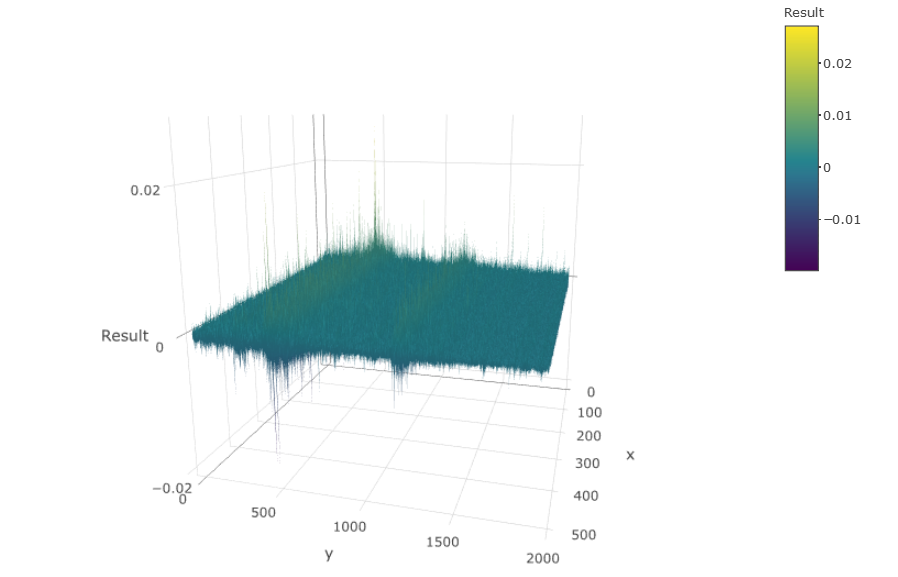
\includegraphics[width=1\textwidth]{BMW_Returns_lattice4.png}
	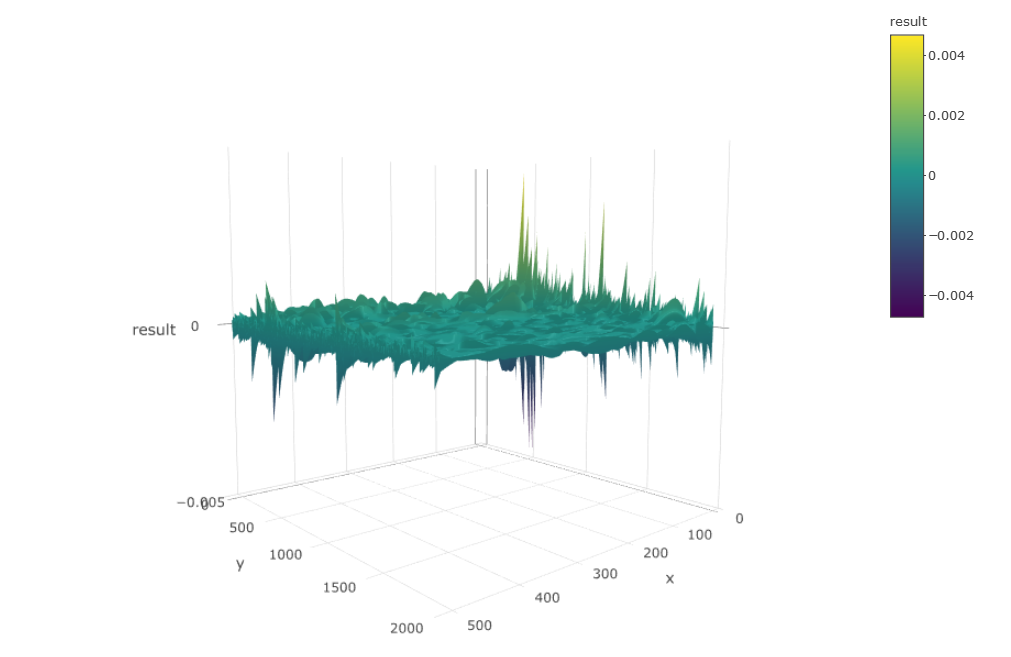
\includegraphics[width=1\textwidth]{BMW_07_14_Ret_trend.png}
	%\decoRule
	\caption{BMW returns and trend 2007 - 2014}
	\label{figure:5.1a}
\end{figure}
\begin{figure}[ht] 
	\centering
	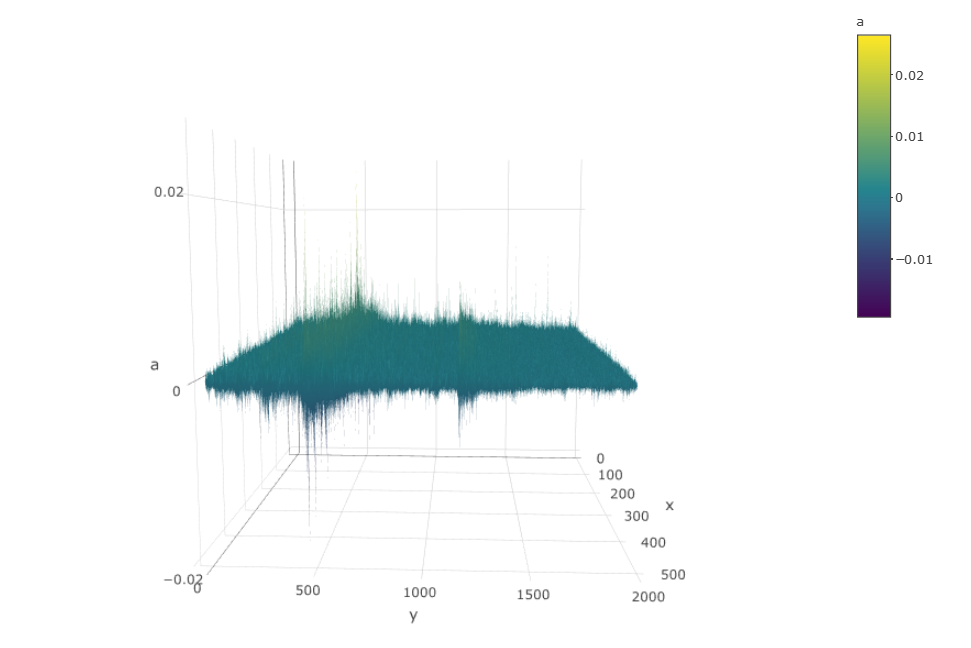
\includegraphics[width=1\textwidth]{BMW_Returns_lattice5.png}
	%\decoRule
	\caption{BMW returns trend adjusted}
	\label{figure:5.1aa}
\end{figure}
Using the return series as input we can specify a surface plot which visualizes the movement of the returns over the course of the trading day 
%since higher trading activity is correlated to market opening and closing times. 
and shows its path across the years along the second horizontal axis. The approach that is necessary to generate figure \ref{figure:5.1a} comes with restructuring the chronological data and its time order. All consecutive 511 trading minutes of the trading day are captured on the x axis, the trading day of 250 days in a year on the y axis and the corresponding return value is given on the z axis. Once the trend in both directions can be calculated we can also receive the trend adjusted residuals or returns. The trend surface for the BMW returns is also given in figure \ref{figure:5.1a}. Subtracting the trend produces the desired stationary short (long) memory lattice process without a deterministic or stochastic trend given in \ref{figure:5.1aa}. 
%\begin{figure}[ht] 
%	\centering
%	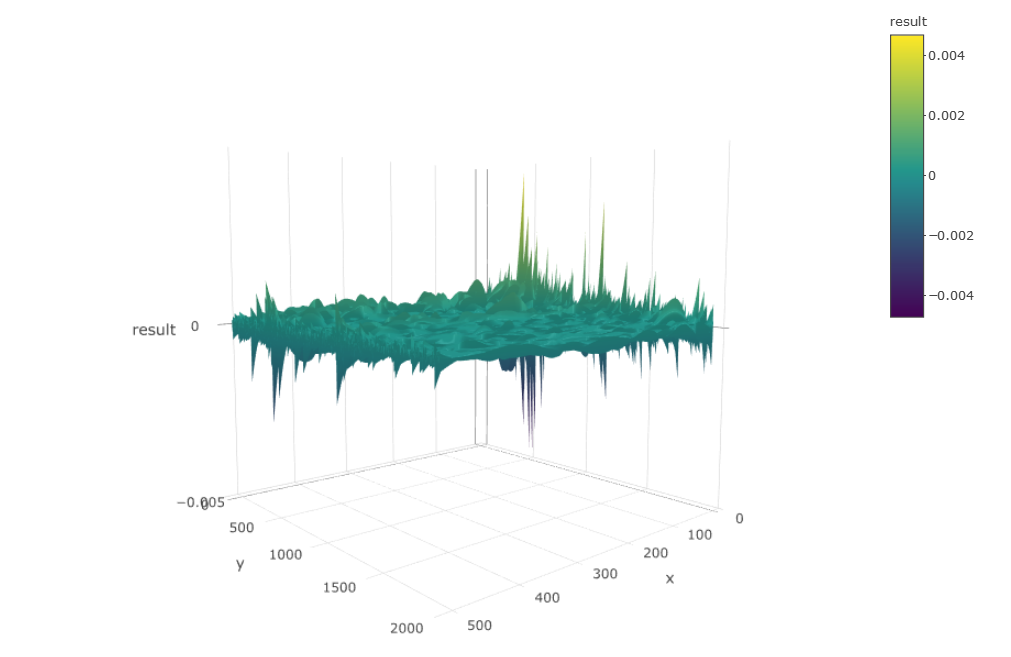
\includegraphics[width=1\textwidth]{BMW_07_14_Ret_trend.png}
%	%\decoRule
%	\caption{BMW trend in returns}
%	\label{figure:5.1aa}
%\end{figure}

\subsection{Over given trading days}
\label{tradingdays}
Trend investigation requires a time series with sufficiently many observations in order to apply a long memory approach. Here BMW returns between the period of January 2007 and July 2014 are represented. The time-in-the-day dimension is used to illustrate the trend behavior against the typical pattern of higher trading activity associated to market opening and closing times. Te returns show a peak in then end of 2008 and in 2011 across all time-in-the-day observations. We investigate the trend mechanisms in each direction separately. 
Three of the almost 2000 trading days of BMW returns are selected and shown in figure \ref{figure:5.1b}. 
%\pagebreak 
\begin{figure}[ht] 
	\centering
	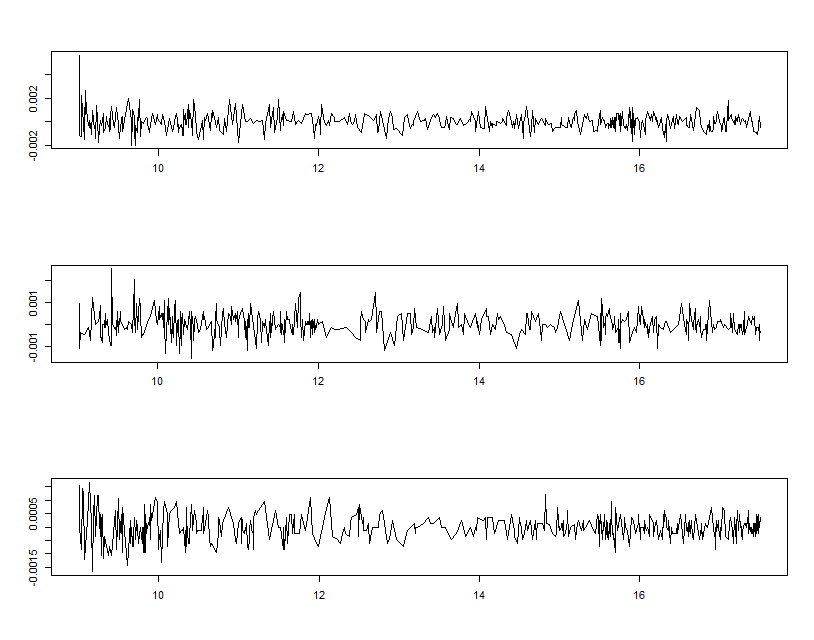
\includegraphics[width=1\textwidth]{Ret_trading_days_01.png}
	%\decoRule
	\caption{BMW returns trading days 2007 - 2014}
	\label{figure:5.1b}
\end{figure}
%\begin{figure}[ht] 
%	\centering
%	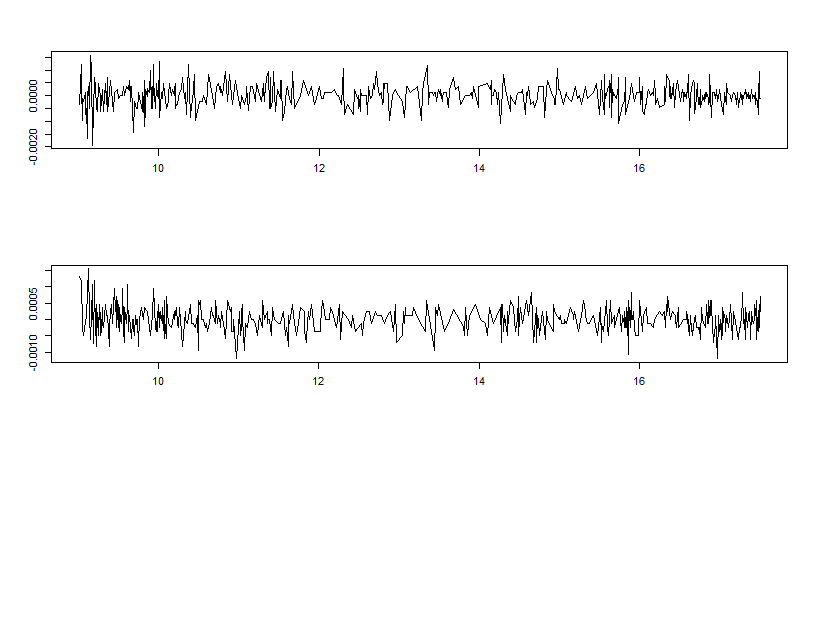
\includegraphics[width=1\textwidth]{Ret_trading_days_02.png}
%	%\decoRule
%	\label{figure:5.1c}
%\end{figure}
%\linebreak
Neglecting the absolute values of the returns the density of the trading activity is visibly at lowest levels during 12 am and 2 pm. Higher trading activity expressed as volatility clustering of the return values can be observed towards market opening and closing times. The chosen \(k\)th value at midday is apparently more distant to its previous value since fewer trading activities lead to fewer ticks between 12 and 2 pm and therefore reduce the density of the volatility. This phenomenon is referred to as the saddle pattern. 
%Therefore, the third dimension time of the day is introduced in addition to time of the year and volume level.  
%Considering the trading times 
%in \ref{tradingtimes} 
%of the trading days will form the lattice process following a S-SEMIFAR model which reveals the trend of the series in day-of-the-year-time direction.  
\subsection{Over given trading times}
\label{tradingtimes}
The dataset is additionally investigated regarding the trading times over a day such that the first minute of the first trading day is followed by the first minute of all considered trading days, thereafter follows the second minute of the first, second and third day and so on. 
The restructuring of the data allows trend investigation while simultaneously accounting for the daily saddle pattern. Two of 510 trading minutes were selected and show the BMW returns of 8 years of trading in figure \ref{figure:5.3}.\\
\\
\begin{figure}[htbp] 
	\centering
	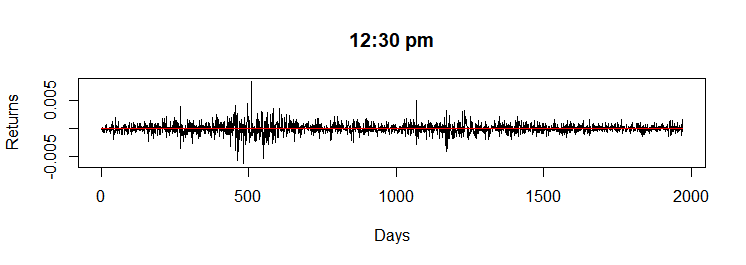
\includegraphics[width=1\textwidth]{Ret_trading_times_03.png}
%	\decoRule
	\label{figure:5.1}
\end{figure}
\begin{figure}[htbp] 
	\centering
	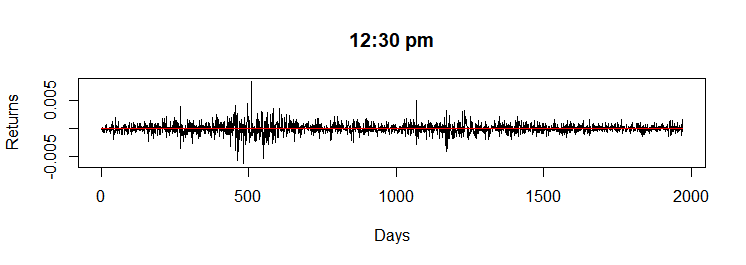
\includegraphics[width=1\textwidth]{Ret_trading_times_03.png}
%	\decoRule
	\caption[BMW]{BMW price day time series}
	\label{figure:5.2}
\end{figure}
\begin{figure}[htbp] 
	\centering
	
	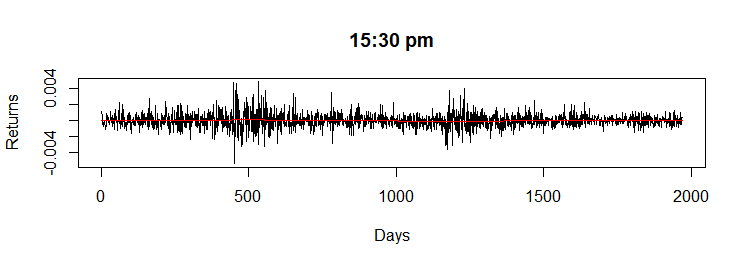
\includegraphics[width=1\textwidth]{Ret_trading_times_05.png}
%	\decoRule
	\caption[BMW]{BMW price day time series}
	\label{figure:5.3}
\end{figure}
\linebreak
Notice the two peaks in returns in 2008 during the financial crises and in the year of sales record 2011. Both irregularities have also been shown in figure \ref{figure:5.1a} and indicate a period of high return volatility.
The spatial SEMIFAR allows the separation of a trend and stationary short- and long- memory component. By subtracting the trend from the returns

\section{Conclusion/Final remarks}
Reviewing the conducted work we conclude, that

%---------------------------------------------------------------------------------------
%	BIBLIOGRAPHY
%---------------------------------------------------------------------------------------

\printbibliography[heading=bibintoc]

%---------------------------------------------------------------------------------------

\end{document}
